\chapterimage{head2.png} % Chapter heading image
\chapter{Hidden Markov Model}
\section{Graphical Model}
\begin{definition}
We denote a particular configuration as $(\textbf{x}, \textbf{y})$
\begin{equation}
(\textbf{x}, \textbf{y})=(x_0, x_1, \cdots, x_T, y_0, y_1, \cdots, y_T)
\end{equation}
\end{definition}

\begin{definition}[The joint probability]
\begin{equation}
p(\textbf{x}, \textbf{y})= p(x_0)\prod_{t=0}^{T-1} p(x_{t+1}|x_t) \prod_{t=0}^{T}p(y_t|x_t)
\end{equation}
\end{definition}
\begin{center}
        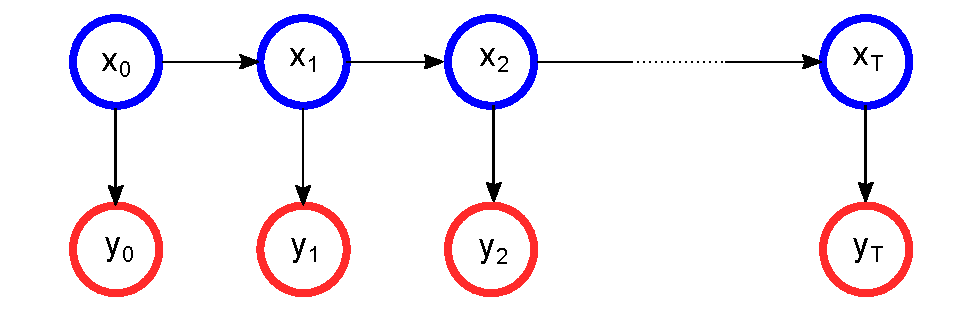
\includegraphics[scale=0.8]{ch2/graphical.pdf}   
\end{center}

\section{Log-likelihood}
We will use the following four states model to illustrate how we calculate the log-likelihood.
\begin{center}
        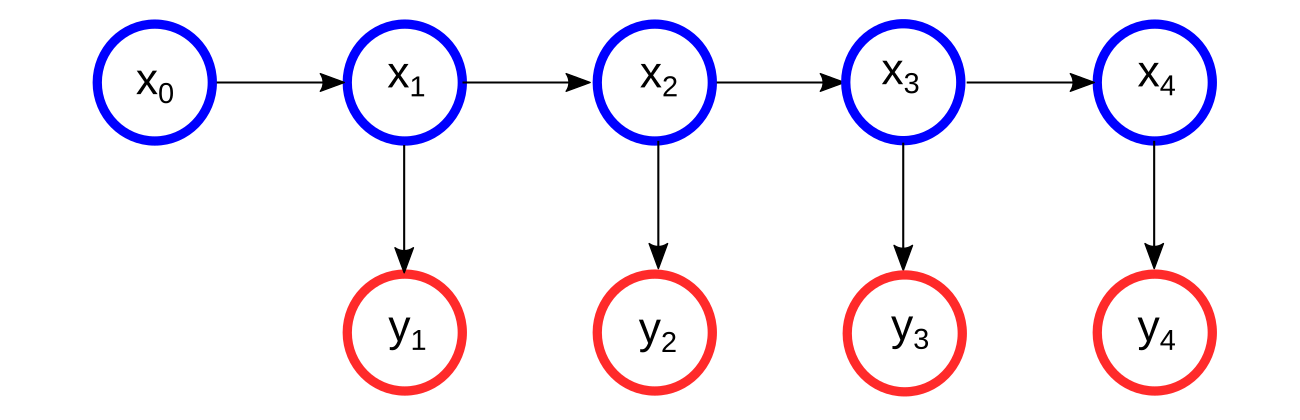
\includegraphics[scale=0.8]{ch2/four_states_ex.png}   
\end{center}

\begin{definition}[$\left< \hat{\alpha}_{t_0} \right|$]
Since there is no external forces, the initial state, $\left< \hat{\alpha}_{t_0} \right|$, is assumed to follow the equilibrium distribution $\rho_{eq}(x)=\sqrt{p_{eq}(x)}$, that is
\begin{equation}
        \left< \alpha_{t_0} | x \right> = \rho_{eq}(x)
\end{equation}
\begin{center}
        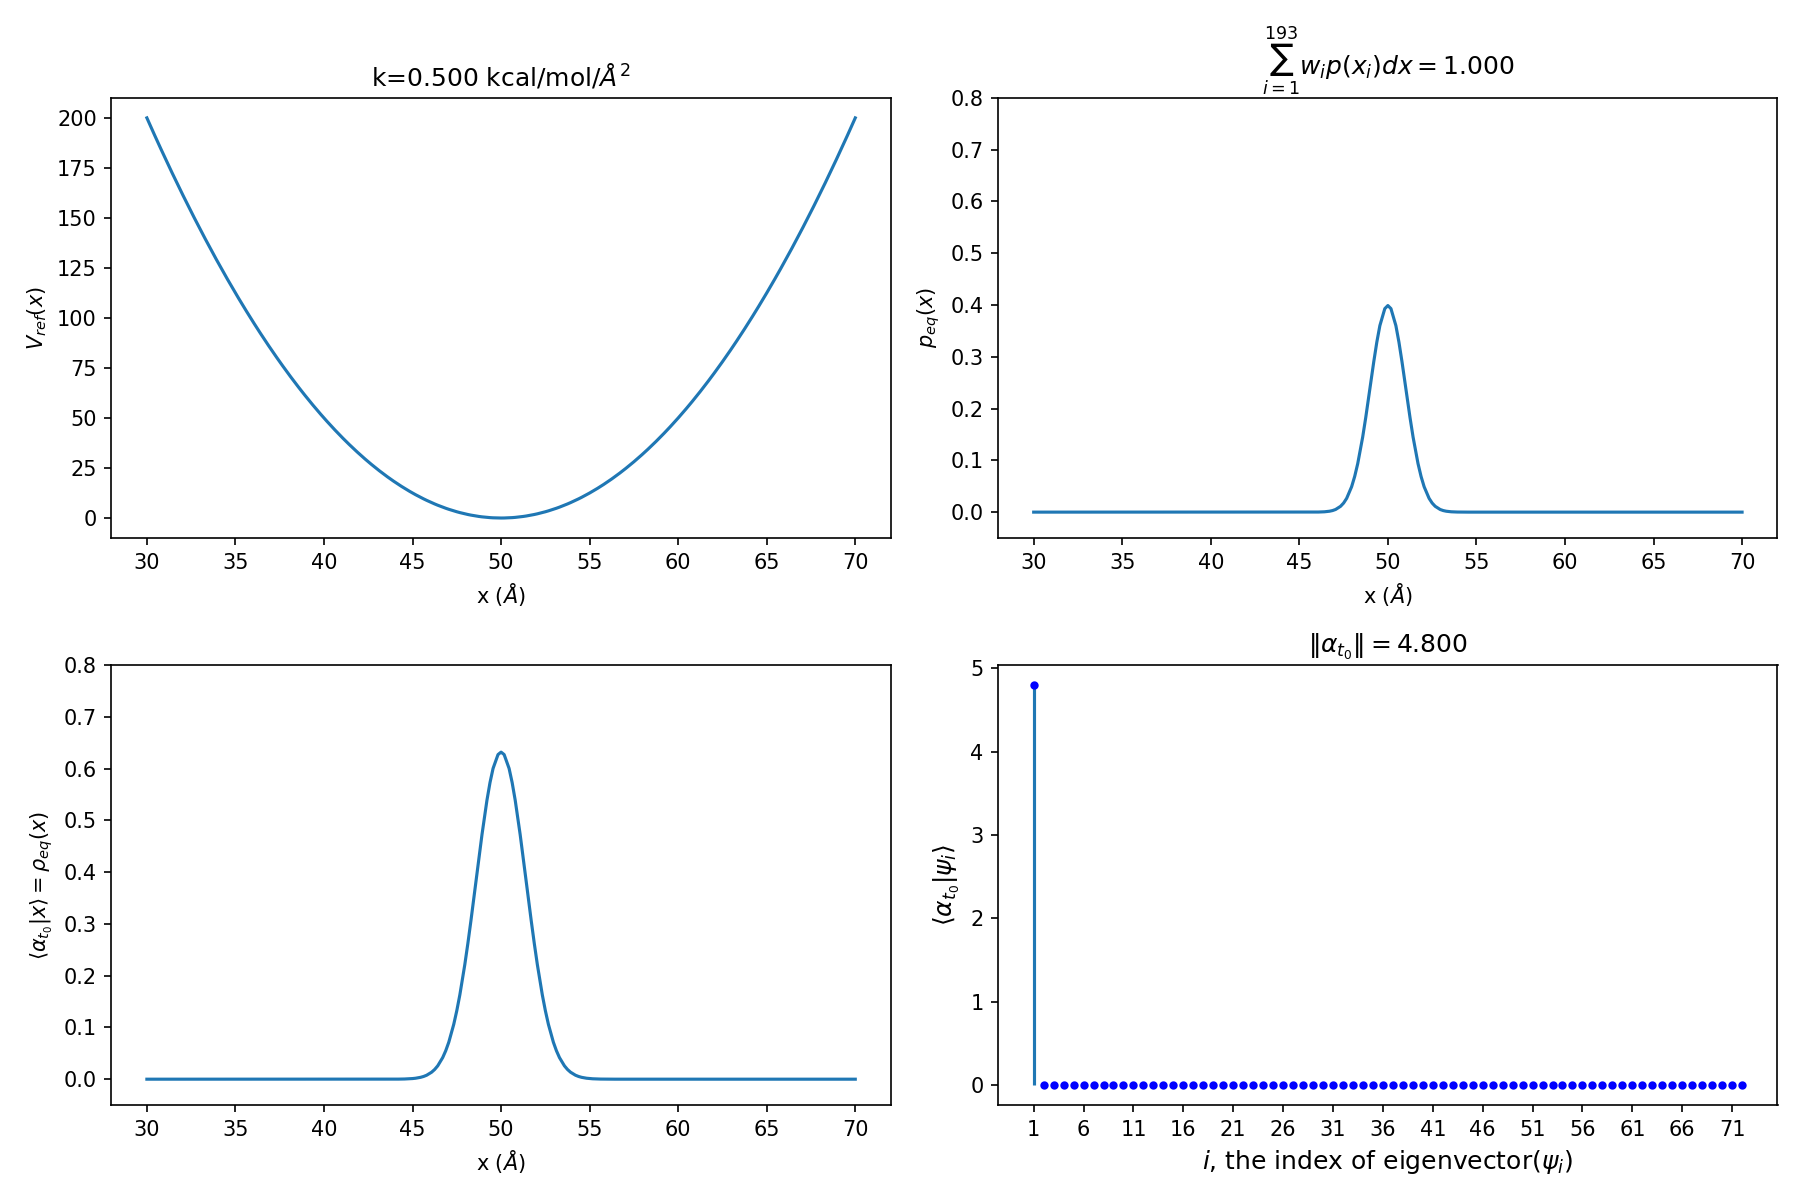
\includegraphics[scale=0.45]{ch2/alpha_t0.png}   
\end{center}
And we know
\begin{align*}
        p(x,t=0) &= \rho_{eq}(x) \rho_{eq}(x)\\
        &= \rho_{eq}(x)[a_{1}(0) \psi_1(x)+a_{2}(0)\psi_2(x)+\cdots+a_{72}(0)\psi_{72}(x)]       
\end{align*}
$\left< \alpha_{t_0} \right|$ is a vector, which is shown in the right-bottom figure.
\begin{equation}
        \left< \alpha_{t_0} \right| = \begin{bmatrix}\left< \alpha_{t_0} | \psi_1 \right> & \left< \alpha_{t_0} | \psi_2 \right> & \cdots & \left< \alpha_{t_0} | \psi_{72} \right> \end{bmatrix}
\end{equation}
and the norm of $\left< \alpha_{t_0} \right|$
\begin{equation}
        \norm{\alpha_{t_0}} = \sqrt{a_{1}^2(0) + a_{2}^2(0) + \cdots + a_{36}^2(0)}       
\end{equation}
Furthermore, note that
\begin{equation}
        \left< \hat{\alpha}_{t_0} \right| = \frac{\left< \alpha_{t_{0}} \right|}{\norm{\alpha_{t_{0}}}} = \left< \alpha_{t_{0}} \right|
\end{equation}
because $\norm{\alpha_{t_0}} = 1$
\end{definition}

\begin{definition}[$\rho(x, t=\Delta t) = \left<\alpha_{t_0}| e^{-\textbf{H}\Delta t}|x \right>$]
\begin{align*}
        &p(x,t=\Delta t) = \rho_{eq}(x) \rho(x, \Delta t)\\
        &= \rho_{eq}(x)[a_{1}(0) \exp{(-\lambda_{1}\Delta t)}\psi_1(x)+a_{2}(0)\exp{(-\lambda_{2}\Delta t)}\psi_2(x)+\cdots+a_{72}(0)\exp{(-\lambda_{72}\Delta t)}\psi_{72}(x)]  \\
        &=  \rho_{eq}(x)[a_{1}(0)\psi_1(x)+a_{2}(0)\exp{(-\lambda_{2}\Delta t)}\psi_2(x)+\cdots+a_{72}(0)\exp{(-\lambda_{72}\Delta t)}\psi_{72}(x)]  
\end{align*}
where $\lambda_1 = 0$
\end{definition}

\begin{definition}[$\left< \hat{\alpha}_{t_1}\right|$]
\begin{equation}
        \left< \alpha_{t_1} \right| = \left< \alpha_{t_0} \right| e^{-\textbf{H} \Delta t} \textbf{y}_1     
\end{equation}
\begin{equation}
        \left< \hat{\alpha}_{t_1} \right| = \frac{\left< \alpha_{t_0} \right| e^{-\textbf{H}\Delta t} \textbf{y}_1}{\norm{\left< \alpha_{t_0} \right| e^{-\textbf{H}\Delta t} \textbf{y}_1}} = \frac{\left< \alpha_{t_{1}} \right|}{\norm{\alpha_{t_{1}}}}
\end{equation}
\begin{center}
        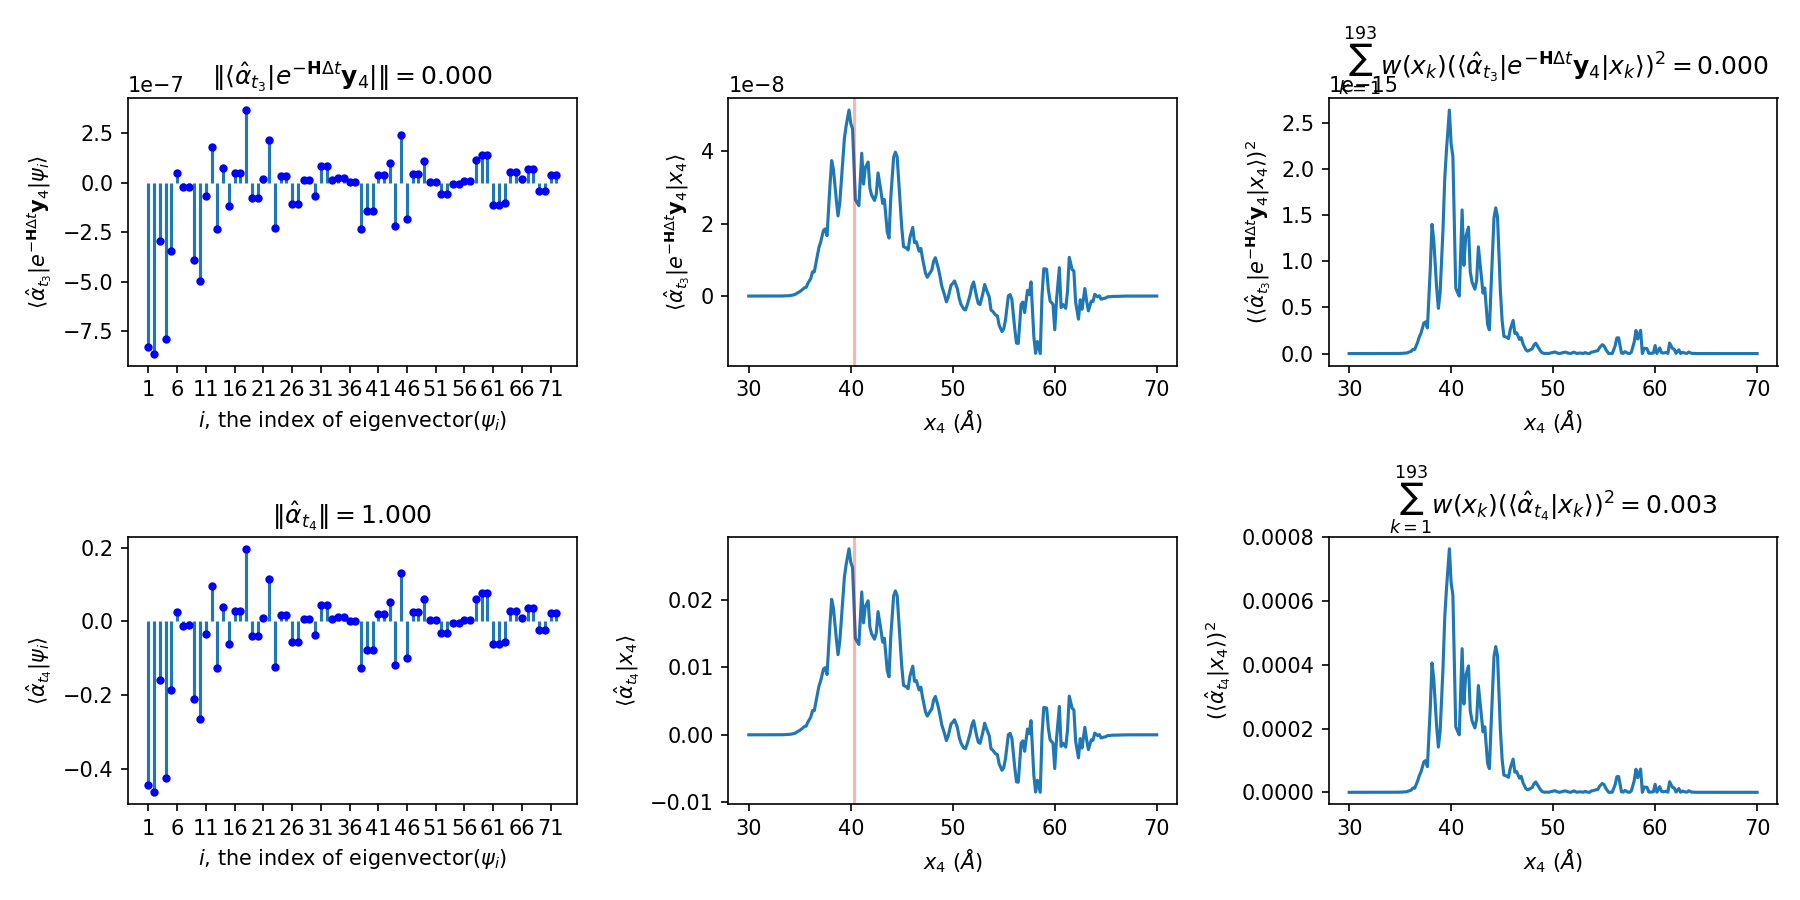
\includegraphics[scale=0.3]{ch2/alpha_1.png}   
\end{center}
\end{definition}

\begin{definition}[$\left< \hat{\alpha}_{t_2}\right|$]
\begin{equation}
        \left< \alpha_{t_2} \right| = \left< \alpha_{t_1} \right| e^{-\textbf{H}\Delta t} \textbf{y}_2     
\end{equation}
\begin{equation}
        \left< \hat{\alpha}_{t_2} \right| 
	= \frac{\left< \hat{\alpha}_{t_1} \right| e^{-\textbf{H}\Delta t} \textbf{y}_2}{\norm{\left< \hat{\alpha}_{t_1} \right| e^{-\textbf{H}\Delta t} \textbf{y}_2}} 
	= \frac{1}{\norm{\alpha_{t_{1}}}} \frac{\left< \alpha_{t_1} \right| e^{-\textbf{H}\Delta t} \textbf{y}_2}{\norm{\left< \hat{\alpha}_{t_1} \right| e^{-\textbf{H}\Delta t} \textbf{y}_2}} 
	= \frac{1}{\norm{\alpha_{t_{1}}}} \frac{1}{\norm{\left< \hat{\alpha}_{t_1} \right| e^{-\textbf{H}\Delta t} \textbf{y}_2}} \left< \alpha_{t_2} \right| 
	= \frac{1}{\norm{\alpha_{t_2}}} \left< \alpha_{t_2} \right|
\end{equation}
where
\begin{equation}
        \norm{\alpha_{t_2}} = \norm{\alpha_{t_{1}}} \norm{\left< \hat{\alpha}_{t_1} \right| e^{-\textbf{H}\Delta t} \textbf{y}_2} 
	= \norm{\left < \hat{\alpha}_{t_{0}} \right| e^{-\textbf{H}\Delta t} \textbf{y}_1} \norm{\left< \hat{\alpha}_{t_1} \right| e^{-\textbf{H}\Delta t} \textbf{y}_2}
\end{equation}
\begin{center}
        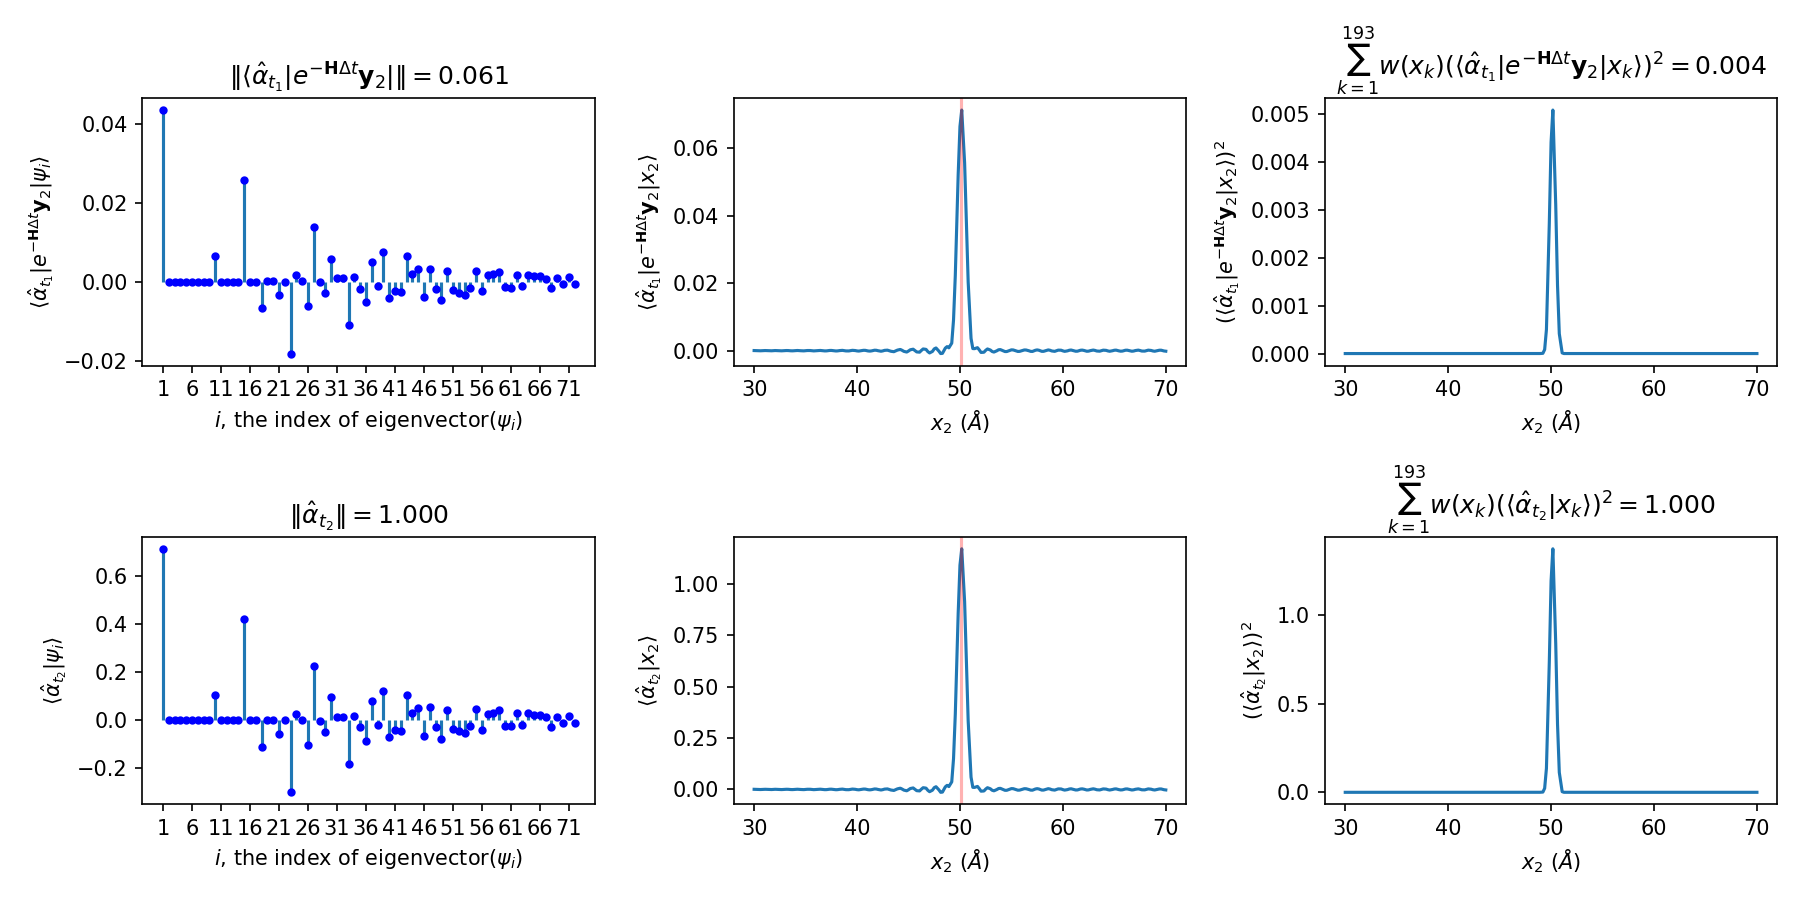
\includegraphics[scale=0.3]{ch2/alpha_2.png}   
\end{center}
\end{definition}

\begin{definition}[$\left< \hat{\alpha}_{t_3}\right|$]
\begin{equation}
        \left< \alpha_{t_3} \right| = \left< \alpha_{t_2} \right| e^{-\textbf{H}\Delta t} \textbf{y}_3               
\end{equation}
\begin{equation}
        \left< \hat{\alpha}_{t_3} \right| 
	= \frac{\left< \hat{\alpha}_{t_2} \right| e^{-\textbf{H}\Delta t} \textbf{y}_3}{\norm{\left< \hat{\alpha}_{t_2} \right| e^{-\textbf{H}\Delta t} \textbf{y}_3}} 
	= \frac{1}{\norm{\alpha_{t_{2}}}} \frac{\left< \alpha_{t_2} \right| e^{-\textbf{H}\Delta t} \textbf{y}_3}{\norm{\left< \hat{\alpha}_{t_2} \right| e^{-\textbf{H}\Delta t} \textbf{y}_3}} 
	= \frac{1}{\norm{\alpha_{t_3}}} \left< \alpha_{t_3} \right|
\end{equation}
where
\begin{equation}
        \norm{\alpha_{t_3}} = \norm{\alpha_{t_{2}}} \norm{\left< \hat{\alpha}_{t_2} \right| e^{-\textbf{H}\Delta t} \textbf{y}_3} 
        = \norm{\left < \hat{\alpha}_{t_{0}} \right| e^{-\textbf{H}\Delta t} \textbf{y}_1} \norm{\left< \hat{\alpha}_{t_1} \right| e^{-\textbf{H}\Delta t} \textbf{y}_2} \norm{\left < \hat{\alpha}_{t_{2}} \right| e^{-\textbf{H}\Delta t} \textbf{y}_3}    
\end{equation}
\begin{center}
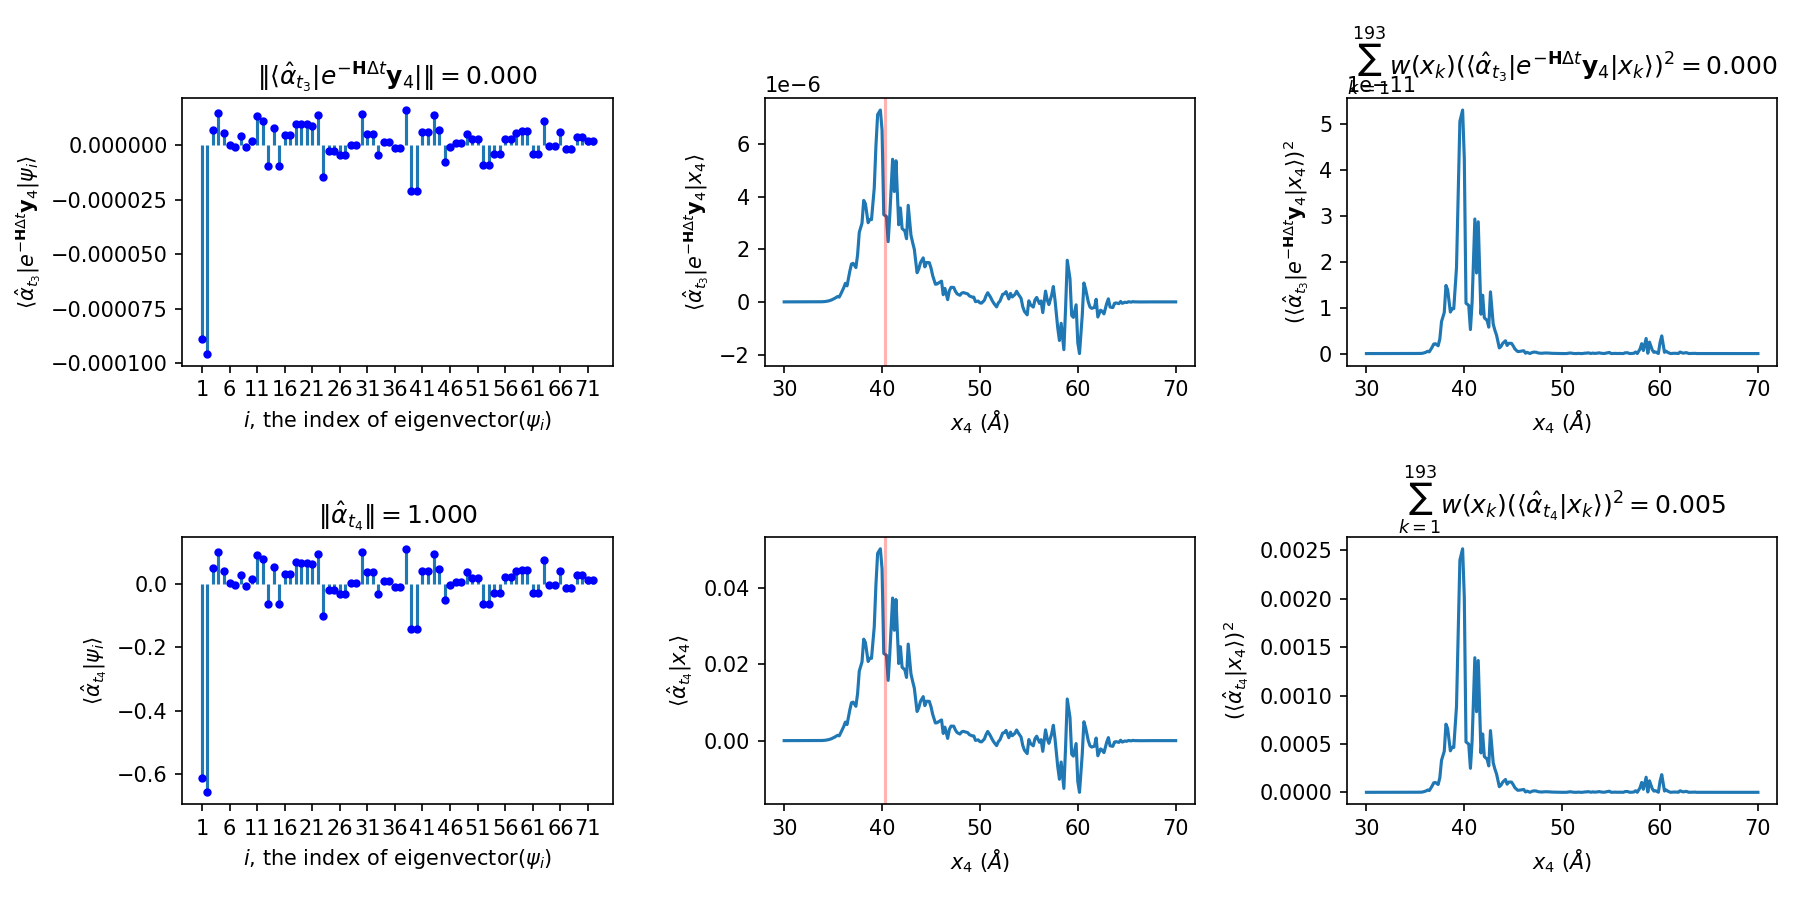
\includegraphics[scale=0.3]{ch2/alpha_3.png}
\end{center}
\end{definition}

\begin{definition}[$\left< \hat{\alpha}_{t_4}\right|$]
\begin{equation}
        \left< \alpha_{t_4} \right| = \left< \alpha_{t_3} \right| e^{-\textbf{H}\Delta t} \textbf{y}_4
\end{equation}
\begin{equation}
        \left< \hat{\alpha}_{t_4} \right| 
	= \frac{\left< \hat{\alpha}_{t_3} \right| e^{-\textbf{H}\Delta t} \textbf{y}_4}{\norm{\left< \hat{\alpha}_{t_3} \right| e^{-\textbf{H}\Delta t} \textbf{y}_4}} 
        = \frac{1}{\norm{\alpha_{t_{3}}}} \frac{\left< \alpha_{t_3} \right| e^{-\textbf{H}\Delta t} \textbf{y}_4}{\norm{\left< \hat{\alpha}_{t_3} \right| e^{-\textbf{H}\Delta t} \textbf{y}_4}} 
        = \frac{1}{\norm{\alpha_{t_4}}} \left< \alpha_{t_4} \right|
\end{equation}
where
\begin{align*}
        \norm{\alpha_{t_4}} &= \norm{\alpha_{t_{3}}} \norm{\left< \hat{\alpha}_{t_3} \right| e^{-\textbf{H}\Delta t} \textbf{y}_4}\\
	&= \norm{\left < \hat{\alpha}_{t_{0}} \right| e^{-\textbf{H}\Delta t} \textbf{y}_1} \norm{\left< \hat{\alpha}_{t_1} \right| e^{-\textbf{H}\Delta t} \textbf{y}_2} \norm{\left < \hat{\alpha}_{t_{2}} \right| e^{-\textbf{H}\Delta t} \textbf{y}_3} \norm{\left < \hat{\alpha}_{t_{3}} \right| e^{-\textbf{H}\Delta t} \textbf{y}_4}
\end{align*}
\begin{center}
        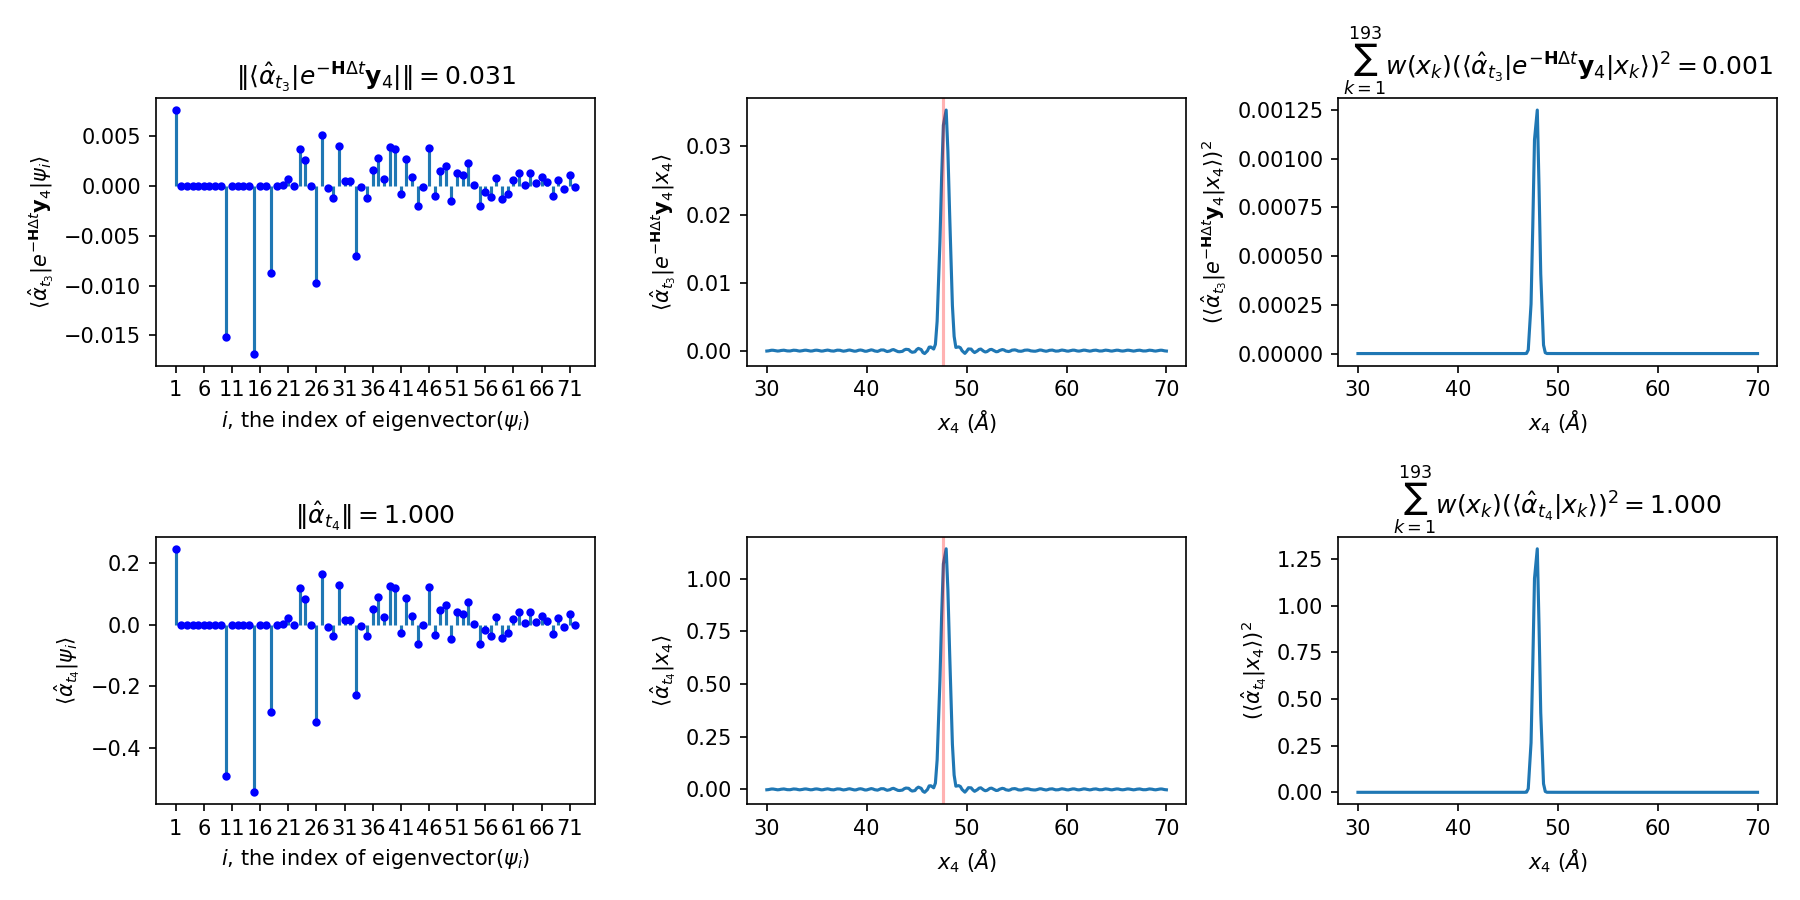
\includegraphics[scale=0.3]{ch2/alpha_4.png}
\end{center}
\end{definition}

\begin{definition}[$\left | \hat{\beta}_{t_4} \right > $]
And the final one is
\begin{center}
        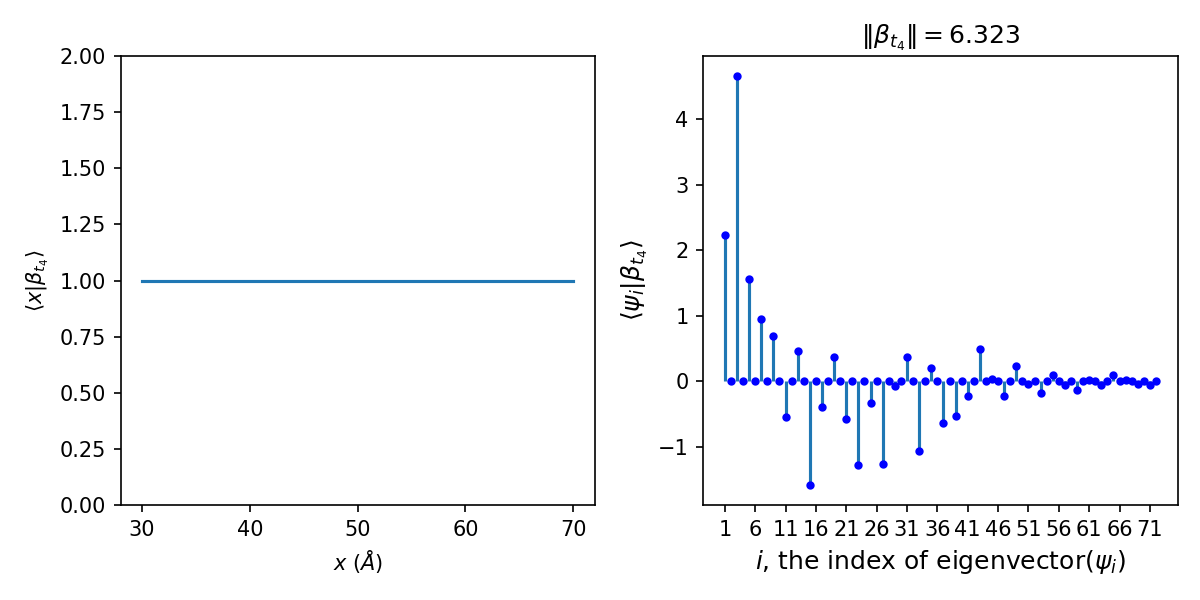
\includegraphics[scale=0.3]{ch2/beta_4.png}
\end{center}
\end{definition}

\begin{definition}[Likelihood functional]
\begin{align*}
        \mathcal{P}(Y(t) ; F(x),D) &= \mathcal{P}(Y(t) ; \theta)= \mathcal{L}[\theta] \\
	&= \langle \alpha_{t_0} |e^{-\textbf{H}\Delta t_1}\textbf{y}_1e^{-\textbf{H}\Delta t_2}\textbf{y}_2 e^{-\textbf{H}\Delta t_{3}}\textbf{y}_{3} e^{-\textbf{H}\Delta t_{4}}\textbf{y}_{4} | \beta_{t_{4}} \rangle \\
	&=  \left < \alpha_{t_{4}} | \beta_{t_{4}} \right > = \norm{\alpha_{t_{4}}} \left < \hat{\alpha}_{t_{4}} | \beta_{t_{4}} \right > 
\end{align*}
\end{definition}

\begin{definition}[Log-likelihood functional]
\begin{align*}
        \ell[\theta] &= \ln \mathcal{L}[\theta] = \ln{\norm{\alpha_{t_{4}}}} + \ln{\left < \hat{\alpha}_{t_{4}} | \beta_{t_{4}} \right >} \\  
        & =2 \sum_{i=1}^{4} \ln{\frac{\norm{\alpha_{t_{i}}}}{\norm{\alpha_{t_{i-1}}}}} + \ln{\frac{ \left < \alpha_{t_{4}} | \beta_{t_{4}}\right>}{\norm{\alpha_{t_{4}}}}} \\ 
        & = 2 \sum_{i=1}^{4} \ln{\norm{\left< \hat{\alpha}_{t_{i-1}} \right| e^{-\textbf{H}\Delta t} \textbf{y}_i}} + \ln{\left < \hat{\alpha}_{t_{4}} | \beta_{t_{4}} \right >} 
\end{align*}
\end{definition}